\documentclass[tikz]{standalone}

\usepackage{pgfplots}
\pgfplotsset{compat=newest}

\usepackage{tkz-tab}
\usepackage{amsmath}

\begin{document}

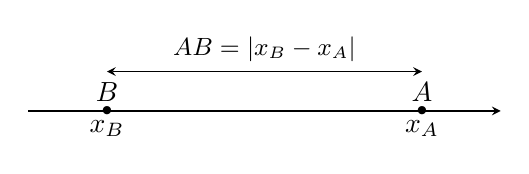
\begin{tikzpicture}
	\draw (-3,0) node {\scriptsize$\bullet$} node[anchor=south] {$B$} node[anchor=north] {$x_B$} coordinate (ae);
	\draw (1,0) node {\scriptsize$\bullet$} node[anchor=south] {$A$} node[anchor=north] {$x_A$} coordinate (ea);
	\draw[->,>=stealth] (-4,0) -- (2,0);
	\draw[<->,>=stealth] (-3,0.5) -- (1,0.5) node[midway,anchor=south] {\small$AB=\lvert x_B-x_A \rvert$};
\end{tikzpicture}

\end{document}